\documentclass{article}

\usepackage{ragged2e} % For justified text alignment
\setlength{\parindent}{0pt} % Remove paragraph indentation

% Language setting
% Replace `english' with e.g. `spanish' to change the document language
\usepackage[english]{babel}

% Set page size and margins
% Replace `letterpaper' with `a4paper' for UK/EU standard size
\usepackage[letterpaper,top=2cm,bottom=2cm,left=3cm,right=3cm,marginparwidth=1.75cm]{geometry}

% Useful packages
\usepackage{amsmath}
\usepackage{graphicx}
\usepackage[colorlinks=true, allcolors=blue]{hyperref}
\onecolumn
\title{A Case of Study for Classifications Algorithm to a Tabular Vector Borne Disease Dataset}
\author{Alberto Arath Figueroa Salomon}
\twocolumn
\begin{document}
\maketitle

\section{Introduction}

Vector-borne diseases have become relevant because human activity
creates imbalance in ecosystems, and this family of diseases has become a recurring problem in warm climates. These diseases have a common set features, in addition to the fact that they are transmitted bites of a blood-sucking arthropod.

Such common features are the prognosis, where the symptoms between each other could be almost indistinguishable 

The purpose of the study is to build a machine learning model that can discern classification patterns for each set of shared symptoms.

\section{Data}

\subsection{Instance composition}
Data set is composed by labeled data, 707 rows and 64 features.
Training data has a synthetic origin so there is really no need for data preparation
which is good as we can focus solely in the application of Machine Learning techniques

% Table environment

\begin{table}[h!] % Single-column table
\centering
\renewcommand{\arraystretch}{1.2} % Adjust row spacing slightly
\scalebox{0.8}{ % Scale to 80% including caption
\begin{tabular}{|c|c|c|c|}
\hline
\textbf{Muscle Pain} & \textbf{Fatigue} & \textbf{Weakness} & \textbf{Prognosis} \\ \hline
Present              & Not Present      & Present           & Present            \\ \hline
Not Present          & Not Present      & Present           & Present            \\ \hline
\end{tabular}
} % End of scaling
\caption{Sample training set with a subset of features.}
\label{tab:sample_training}
\end{table}
\subsection{Predictor Set}
Is composed of binary variables specifying if given symptom is present 
in this prognosis instance it represents the presence or absence of a specific condition, The variable \( X \) takes values from the set:
\[
X \in \{0, 1\},
\]
where:
\[
X =
\begin{cases}
1 & \text{if the condition is \textbf{present}}, \\
0 & \text{if the condition is \textbf{not present}}.
\end{cases}
\]

\subsection{Target Variable}
The target variable is called Prognosis containing the Vector-borne dissease classfier

The target variable, denoted as \( Y \), is a categorical variable representing the prognosis outcome it can take values from the following finite set of classes:

\[
Y \in \{ C_1, C_2, \dots, C_k \},
\] 
where \( C_i \) represents the \( i^{\text{th}} \) class label, for \( i = 1, 2, \dots, k \).

In this study, \( k = 11 \), and the classes are defined as follows:
\begin{itemize}
    \item \( C_1 \): Dengue,
    \item \( C_2 \): Zika,
    \item \( C_3 \): Malaria.
\end{itemize}
To allow the application of machine learning algorithms label encoder variables as in following example
\[
Y = 
\begin{cases} 
0 & \text{if the class is \( C_1 \) (Malaria)}, \\
1 & \text{if the class is \( C_2 \) (Dengue)}, \\
2 & \text{if the class is \( C_3 \) (Zika)}.
\end{cases}
\]
This encoding To allows the application of machine learning algorithms such as softmax regression, decision trees, or neural networks to predict the likelihood of each class based on the input features.

\section{Exploratory Data Analysis (EDA)}

\subsection{Class distribution}

Class distribution shows there is no significan class imbalance,
Figure 1 show West Nile Fever with 80 instances and Malaria falls short with 50
as part of study, class imbalance could have and impact but we expect not be 
signicant. Just for the sake of the study we will apply oversampling techniques
to improve model.

\onecolumn
\begin{figure}[h!]
\centering
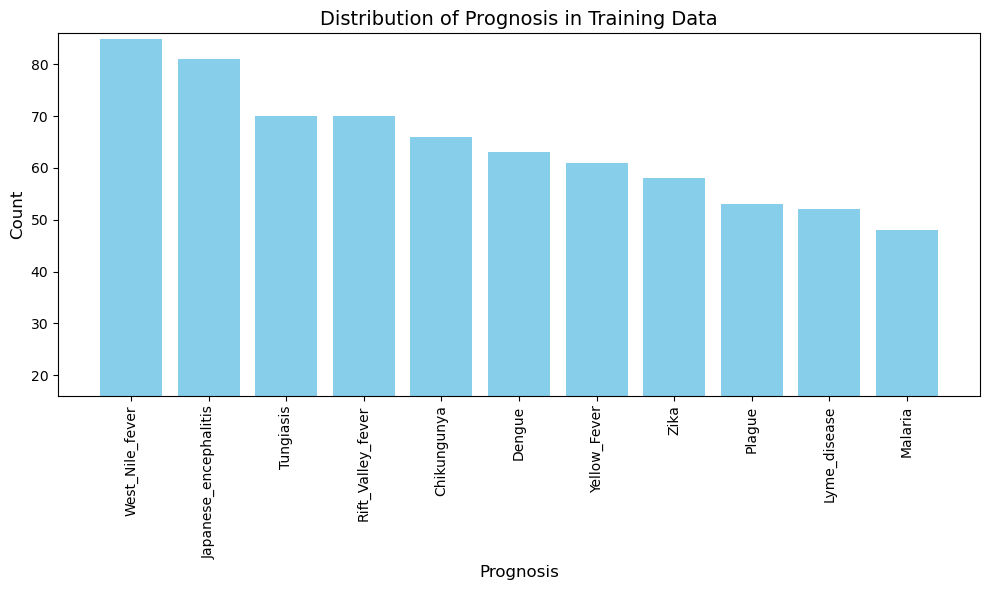
\includegraphics[width=.8\linewidth]{Disease Distribution.png}
\caption{\label{fig:frog}Distribution of Prognosis in Training Data.}
\end{figure}

\twocolumn
\subsection{Features correaltion matrix}
Features 

\onecolumn

\begin{figure}[h!]
\centering
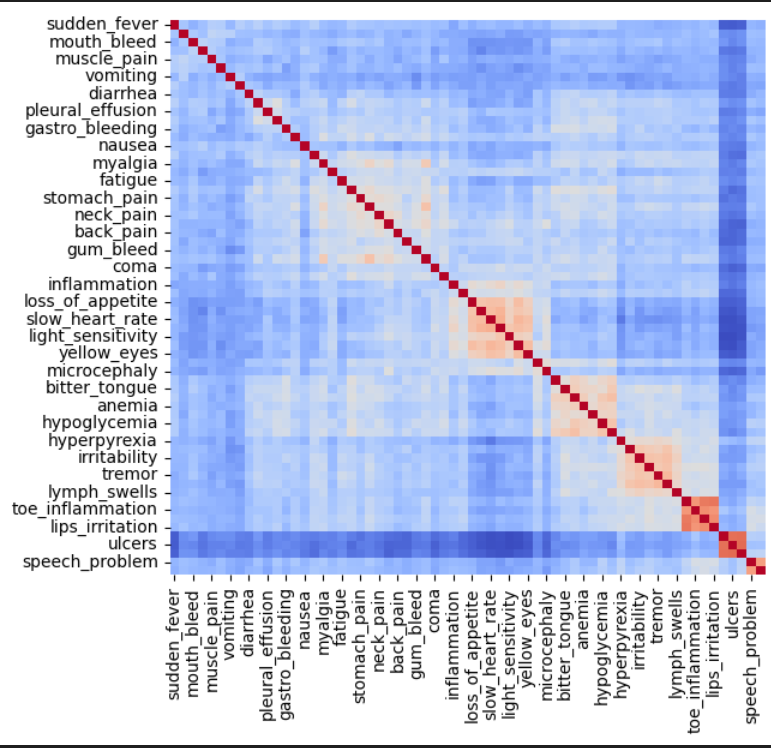
\includegraphics[width=.8\linewidth]{CorrelationMatrix.png}
\caption{\label{fig:frog}Features Correlation Matrix.}
\end{figure}
\twocolumn


\section{Grid search to best find best cross validation precision results}

Track changes are available on all our \href{https://www.overleaf.com/user/subscription/plans}{premium plans}, and can be toggled on or off using the option at the top of the Review pane. Track changes allow you to keep track of every change made to the document, along with the person making the change. 

\subsection{How to add Lists}

You can make lists with automatic numbering \dots

\begin{enumerate}
\item Like this,
\item and like this.
\end{enumerate}
\dots or bullet points \dots
\begin{itemize}
\item Like this,
\item and like this.
\end{itemize}

\section{Grid search to best find best cross validation precision results}

\LaTeX{} is great at typesetting mathematics. Let $X_1, X_2, \ldots, X_n$ be a sequence of independent and identically distributed random variables with $\text{E}[X_i] = \mu$ and $\text{Var}[X_i] = \sigma^2 < \infty$, and let
\[S_n = \frac{X_1 + X_2 + \cdots + X_n}{n}
      = \frac{1}{n}\sum_{i}^{n} X_i\]
denote their mean. Then as $n$ approaches infinity, the random variables $\sqrt{n}(S_n - \mu)$ converge in distribution to a normal $\mathcal{N}(0, \sigma^2)$.


To change the spell check language, simply open the Overleaf menu at the top left of the editor window, scroll down to the spell check setting, and adjust accordingly.


\section{Conclusions}

\bibliographystyle{alpha}
\bibliography{sample}

\end{document}